\setcounter{section}{5}
\section{Basiswechsel und Diagonalisierung}

\subsection{Basiswechsel für Vektoren}

Was bedeutet es nochmal, wenn wir einen Vektor mit den Koordinaten \( \begin{bmatrix} -4 & 1 \end{bmatrix}^\top \) beschreiben? Grundlegend beschreiben Koordinaten um wie viel die Basisvektoren des assoziierten Vektorraums skaliert werden. In der Standardbasis ist dies bereits recht intuitiv. 

\begin{equation*}
    -4 \begin{bmatrix} 1 \\ 0 \end{bmatrix} + 1 \begin{bmatrix} 0 \\ 1 \end{bmatrix} = \begin{bmatrix} -4 \\ 1 \end{bmatrix} 
\end{equation*}

\begin{figure}[h]
    \centering
    \tikzset{every picture/.style={line width=0.75pt}} %set default line width to 0.75pt        
    \begin{tikzpicture}[x=0.75pt,y=0.75pt,yscale=-1,xscale=1]
        %uncomment if require: \path (0,300); %set diagram left start at 0, and has height of 300
        %Straight Lines [id:da2563845726116647] 
        \draw [color={rgb, 255:red, 155; green, 155; blue, 155 }  ,draw opacity=1 ] [dash pattern={on 0.84pt off 2.51pt}]  (410,140) -- (250,140) ;
        %Straight Lines [id:da9238284130224473] 
        \draw [color={rgb, 255:red, 255; green, 255; blue, 255 }  ,draw opacity=1 ]   (310,190) -- (587.03,150.42) ;
        \draw [shift={(590,150)}, rotate = 171.87] [fill={rgb, 255:red, 255; green, 255; blue, 255 }  ,fill opacity=1 ][line width=0.08]  [draw opacity=0] (5.36,-2.57) -- (0,0) -- (5.36,2.57) -- (3.56,0) -- cycle    ;
        %Straight Lines [id:da8899671494545942] 
        \draw [color={rgb, 255:red, 255; green, 255; blue, 255 }  ,draw opacity=1 ][line width=1.5]    (410,175.71) -- (253.99,164.57) ;
        \draw [shift={(250,164.29)}, rotate = 4.09] [fill={rgb, 255:red, 255; green, 255; blue, 255 }  ,fill opacity=1 ][line width=0.08]  [draw opacity=0] (6.43,-3.09) -- (0,0) -- (6.43,3.09) -- (4.27,0) -- cycle    ;

        %Straight Lines [id:da6456313396810407] 
        \draw [color={rgb, 255:red, 0; green, 0; blue, 0 }  ,draw opacity=1 ]   (410,210) -- (410,113) ;
        \draw [shift={(410,110)}, rotate = 90] [fill={rgb, 255:red, 0; green, 0; blue, 0 }  ,fill opacity=1 ][line width=0.08]  [draw opacity=0] (5.36,-2.57) -- (0,0) -- (5.36,2.57) -- (3.56,0) -- cycle    ;
        %Straight Lines [id:da1841211407646408] 
        \draw [color={rgb, 255:red, 0; green, 0; blue, 0 }  ,draw opacity=1 ]   (220,180) -- (517,180) ;
        \draw [shift={(520,180)}, rotate = 180] [fill={rgb, 255:red, 0; green, 0; blue, 0 }  ,fill opacity=1 ][line width=0.08]  [draw opacity=0] (5.36,-2.57) -- (0,0) -- (5.36,2.57) -- (3.56,0) -- cycle    ;
        %Straight Lines [id:da4368708787673843] 
        \draw    (370,175) -- (370,180) ;
        %Straight Lines [id:da7513217910382991] 
        \draw    (330,175) -- (330,180) ;
        %Straight Lines [id:da5860326377427854] 
        \draw    (290,175) -- (290,180) ;
        %Straight Lines [id:da7769871622885531] 
        \draw    (250,175) -- (250,180) ;
        %Straight Lines [id:da6410858500698556] 
        \draw    (450,175) -- (450,180) ;
        %Straight Lines [id:da7768146437339456] 
        \draw    (410,140) -- (405,140) ;
        %Straight Lines [id:da4745392780845308] 
        \draw [color={rgb, 255:red, 74; green, 144; blue, 226 }  ,draw opacity=1 ][line width=1.5]    (410,180) -- (446,180) ;
        \draw [shift={(450,180)}, rotate = 180] [fill={rgb, 255:red, 74; green, 144; blue, 226 }  ,fill opacity=1 ][line width=0.08]  [draw opacity=0] (6.43,-3.09) -- (0,0) -- (6.43,3.09) -- (4.27,0) -- cycle    ;
        %Straight Lines [id:da7230645824561245] 
        \draw [color={rgb, 255:red, 208; green, 2; blue, 27 }  ,draw opacity=1 ][line width=1.5]    (410,180) -- (410,144) ;
        \draw [shift={(410,140)}, rotate = 90] [fill={rgb, 255:red, 208; green, 2; blue, 27 }  ,fill opacity=1 ][line width=0.08]  [draw opacity=0] (6.43,-3.09) -- (0,0) -- (6.43,3.09) -- (4.27,0) -- cycle    ;
        %Straight Lines [id:da7477144553729851] 
        \draw [color={rgb, 255:red, 245; green, 166; blue, 35 }  ,draw opacity=1 ][line width=1.5]    (410,180) -- (253.88,140.97) ;
        \draw [shift={(250,140)}, rotate = 14.04] [fill={rgb, 255:red, 245; green, 166; blue, 35 }  ,fill opacity=1 ][line width=0.08]  [draw opacity=0] (6.43,-3.09) -- (0,0) -- (6.43,3.09) -- (4.27,0) -- cycle    ;
        %Straight Lines [id:da8954129505238868] 
        \draw    (490,175) -- (490,180) ;
        %Straight Lines [id:da7722320016058947] 
        \draw [color={rgb, 255:red, 155; green, 155; blue, 155 }  ,draw opacity=1 ] [dash pattern={on 0.84pt off 2.51pt}]  (250,180) -- (250,140) ;
    \end{tikzpicture}
\end{figure}

Wir können aber auch eine andere Basis wählen, z.B.\ gegeben durch die Vektoren \( \begin{bmatrix} 2 & 1 \end{bmatrix}^\top \) und \( \begin{bmatrix} -1 & 1 \end{bmatrix}^\top \). Wenn wir nun dieselben Koordinaten wie in der Standardbasis benutzten, bekommen wir einen anderen Vektor. 

\begin{equation*}
    -4 \begin{bmatrix} 2 \\ 1 \end{bmatrix} + 1 \begin{bmatrix} -1 \\ 1 \end{bmatrix} = \begin{bmatrix} -7 \\ -3 \end{bmatrix} \neq \begin{bmatrix} -4 \\ 1 \end{bmatrix}
\end{equation*}

\begin{figure}[h]
    \centering
    \tikzset{every picture/.style={line width=0.75pt}} %set default line width to 0.75pt        
    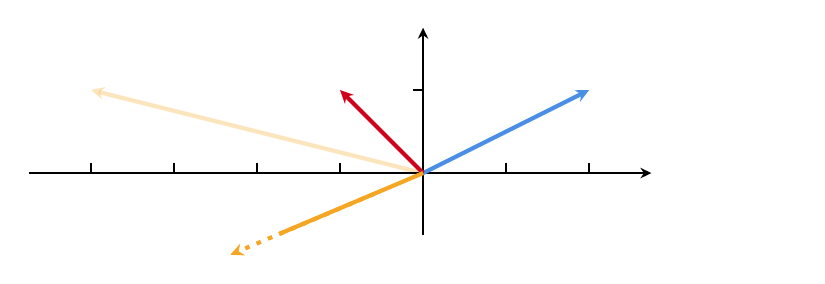
\begin{tikzpicture}[x=0.75pt,y=0.75pt,yscale=-1,xscale=1]
        %uncomment if require: \path (0,300); %set diagram left start at 0, and has height of 300
        
        %Straight Lines [id:da01758312990137323] 
        \draw [color={rgb, 255:red, 245; green, 166; blue, 35 }  ,draw opacity=0.3 ][line width=1.5]    (390,160) -- (233.88,120.97) ;
        \draw [shift={(230,120)}, rotate = 14.04] [fill={rgb, 255:red, 245; green, 166; blue, 35 }  ,fill opacity=0.3 ][line width=0.08]  [draw opacity=0] (6.43,-3.09) -- (0,0) -- (6.43,3.09) -- (4.27,0) -- cycle    ;
        %Straight Lines [id:da4582485034206436] 
        \draw [color={rgb, 255:red, 255; green, 255; blue, 255 }  ,draw opacity=1 ]   (290,190) -- (567.01,170.21) ;
        \draw [shift={(570,170)}, rotate = 175.91] [fill={rgb, 255:red, 255; green, 255; blue, 255 }  ,fill opacity=1 ][line width=0.08]  [draw opacity=0] (5.36,-2.57) -- (0,0) -- (5.36,2.57) -- (3.56,0) -- cycle    ;
        %Straight Lines [id:da029235985874314085] 
        \draw [color={rgb, 255:red, 255; green, 255; blue, 255 }  ,draw opacity=1 ][line width=1.5]    (390,182.86) -- (234,177.29) ;
        \draw [shift={(230,177.14)}, rotate = 2.05] [fill={rgb, 255:red, 255; green, 255; blue, 255 }  ,fill opacity=1 ][line width=0.08]  [draw opacity=0] (6.43,-3.09) -- (0,0) -- (6.43,3.09) -- (4.27,0) -- cycle    ;
        
        %Straight Lines [id:da6456313396810407] 
        \draw [color={rgb, 255:red, 0; green, 0; blue, 0 }  ,draw opacity=1 ]   (390,190) -- (390,93) ;
        \draw [shift={(390,90)}, rotate = 90] [fill={rgb, 255:red, 0; green, 0; blue, 0 }  ,fill opacity=1 ][line width=0.08]  [draw opacity=0] (5.36,-2.57) -- (0,0) -- (5.36,2.57) -- (3.56,0) -- cycle    ;
        %Straight Lines [id:da1841211407646408] 
        \draw [color={rgb, 255:red, 0; green, 0; blue, 0 }  ,draw opacity=1 ]   (200,160) -- (497,160) ;
        \draw [shift={(500,160)}, rotate = 180] [fill={rgb, 255:red, 0; green, 0; blue, 0 }  ,fill opacity=1 ][line width=0.08]  [draw opacity=0] (5.36,-2.57) -- (0,0) -- (5.36,2.57) -- (3.56,0) -- cycle    ;
        %Straight Lines [id:da4368708787673843] 
        \draw    (350,155) -- (350,160) ;
        %Straight Lines [id:da7513217910382991] 
        \draw    (310,155) -- (310,160) ;
        %Straight Lines [id:da5860326377427854] 
        \draw    (270,155) -- (270,160) ;
        %Straight Lines [id:da7769871622885531] 
        \draw    (230,155) -- (230,160) ;
        %Straight Lines [id:da6410858500698556] 
        \draw    (430,155) -- (430,160) ;
        %Straight Lines [id:da7768146437339456] 
        \draw    (390,120) -- (385,120) ;
        %Straight Lines [id:da4745392780845308] 
        \draw [color={rgb, 255:red, 74; green, 144; blue, 226 }  ,draw opacity=1 ][line width=1.5]    (390,160) -- (466.42,121.79) ;
        \draw [shift={(470,120)}, rotate = 153.43] [fill={rgb, 255:red, 74; green, 144; blue, 226 }  ,fill opacity=1 ][line width=0.08]  [draw opacity=0] (6.43,-3.09) -- (0,0) -- (6.43,3.09) -- (4.27,0) -- cycle    ;
        %Straight Lines [id:da7230645824561245] 
        \draw [color={rgb, 255:red, 208; green, 2; blue, 27 }  ,draw opacity=1 ][line width=1.5]    (390,160) -- (352.83,122.83) ;
        \draw [shift={(350,120)}, rotate = 45] [fill={rgb, 255:red, 208; green, 2; blue, 27 }  ,fill opacity=1 ][line width=0.08]  [draw opacity=0] (6.43,-3.09) -- (0,0) -- (6.43,3.09) -- (4.27,0) -- cycle    ;
        %Straight Lines [id:da8954129505238868] 
        \draw    (470,155) -- (470,160) ;
        %Straight Lines [id:da5781004266492847] 
        \draw [color={rgb, 255:red, 245; green, 166; blue, 35 }  ,draw opacity=1 ][line width=1.5]    (390,160) -- (320.67,189.33) ;
        %Straight Lines [id:da13542334227286756] 
        \draw [color={rgb, 255:red, 245; green, 166; blue, 35 }  ,draw opacity=1 ][line width=1.5]  [dash pattern={on 1.69pt off 2.76pt}]  (366.5,170) -- (300.85,197.77) ;
        \draw [shift={(297.17,199.33)}, rotate = 337.07] [fill={rgb, 255:red, 245; green, 166; blue, 35 }  ,fill opacity=1 ][line width=0.08]  [draw opacity=0] (6.43,-3.09) -- (0,0) -- (6.43,3.09) -- (4.27,0) -- cycle    ;
    \end{tikzpicture}
\end{figure}

Mit den neuen Basisvektoren wären die richtigen Koordinaten für denselben Vektor gegeben durch

\begin{equation*}
    -1 \begin{bmatrix} 2 \\ 1 \end{bmatrix} +2 \begin{bmatrix} -1 \\ 1 \end{bmatrix} = \begin{bmatrix} -4 \\ 1 \end{bmatrix}
\end{equation*}

\begin{figure}[h]
    \centering
    \tikzset{every picture/.style={line width=0.75pt}} %set default line width to 0.75pt        
    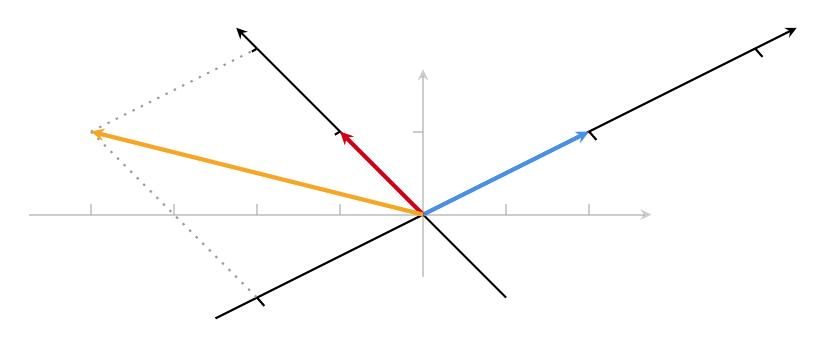
\begin{tikzpicture}[x=0.75pt,y=0.75pt,yscale=-1,xscale=1]
        %uncomment if require: \path (0,300); %set diagram left start at 0, and has height of 300
        
        %Straight Lines [id:da9533695032094103] 
        \draw [color={rgb, 255:red, 155; green, 155; blue, 155 }  ,draw opacity=0.5 ]   (330,135) -- (330,140) ;
        %Straight Lines [id:da917270860192773] 
        \draw [color={rgb, 255:red, 155; green, 155; blue, 155 }  ,draw opacity=0.5 ]   (290,135) -- (290,140) ;
        %Straight Lines [id:da24414341059778377] 
        \draw [color={rgb, 255:red, 155; green, 155; blue, 155 }  ,draw opacity=0.5 ]   (250,135) -- (250,140) ;
        %Straight Lines [id:da5082564391067692] 
        \draw [color={rgb, 255:red, 155; green, 155; blue, 155 }  ,draw opacity=0.5 ]   (210,135) -- (210,140) ;
        %Straight Lines [id:da9120085108269914] 
        \draw [color={rgb, 255:red, 155; green, 155; blue, 155 }  ,draw opacity=0.5 ]   (410,135) -- (410,140) ;
        %Straight Lines [id:da433463449434766] 
        \draw [color={rgb, 255:red, 155; green, 155; blue, 155 }  ,draw opacity=0.5 ]   (370,100) -- (365,100) ;
        %Straight Lines [id:da6549645248390609] 
        \draw [color={rgb, 255:red, 155; green, 155; blue, 155 }  ,draw opacity=0.5 ]   (450,135) -- (450,140) ;
        %Straight Lines [id:da8184570703604538] 
        \draw [color={rgb, 255:red, 155; green, 155; blue, 155 }  ,draw opacity=0.5 ]   (370,170) -- (370,73) ;
        \draw [shift={(370,70)}, rotate = 90] [fill={rgb, 255:red, 155; green, 155; blue, 155 }  ,fill opacity=0.5 ][line width=0.08]  [draw opacity=0] (5.36,-2.57) -- (0,0) -- (5.36,2.57) -- (3.56,0) -- cycle    ;
        %Straight Lines [id:da6755275294719127] 
        \draw [color={rgb, 255:red, 155; green, 155; blue, 155 }  ,draw opacity=0.5 ]   (180,140) -- (477,140) ;
        \draw [shift={(480,140)}, rotate = 180] [fill={rgb, 255:red, 155; green, 155; blue, 155 }  ,fill opacity=0.5 ][line width=0.08]  [draw opacity=0] (5.36,-2.57) -- (0,0) -- (5.36,2.57) -- (3.56,0) -- cycle    ;
        
        
        %Straight Lines [id:da6456313396810407] 
        \draw [color={rgb, 255:red, 0; green, 0; blue, 0 }  ,draw opacity=1 ]   (410,180) -- (282.12,52.12) ;
        \draw [shift={(280,50)}, rotate = 45] [fill={rgb, 255:red, 0; green, 0; blue, 0 }  ,fill opacity=1 ][line width=0.08]  [draw opacity=0] (5.36,-2.57) -- (0,0) -- (5.36,2.57) -- (3.56,0) -- cycle    ;
        %Straight Lines [id:da1841211407646408] 
        \draw [color={rgb, 255:red, 0; green, 0; blue, 0 }  ,draw opacity=1 ]   (270,190) -- (547.32,51.34) ;
        \draw [shift={(550,50)}, rotate = 153.43] [fill={rgb, 255:red, 0; green, 0; blue, 0 }  ,fill opacity=1 ][line width=0.08]  [draw opacity=0] (5.36,-2.57) -- (0,0) -- (5.36,2.57) -- (3.56,0) -- cycle    ;
        %Straight Lines [id:da4745392780845308] 
        \draw [color={rgb, 255:red, 74; green, 144; blue, 226 }  ,draw opacity=1 ][line width=1.5]    (370,140) -- (438.3,105.85) -- (446.42,101.79) ;
        \draw [shift={(450,100)}, rotate = 153.43] [fill={rgb, 255:red, 74; green, 144; blue, 226 }  ,fill opacity=1 ][line width=0.08]  [draw opacity=0] (6.43,-3.09) -- (0,0) -- (6.43,3.09) -- (4.27,0) -- cycle    ;
        %Straight Lines [id:da45268054019438253] 
        \draw [color={rgb, 255:red, 155; green, 155; blue, 155 }  ,draw opacity=1 ] [dash pattern={on 0.84pt off 2.51pt}]  (210,100) -- (290,180) ;
        %Straight Lines [id:da36925602550777736] 
        \draw [color={rgb, 255:red, 155; green, 155; blue, 155 }  ,draw opacity=1 ] [dash pattern={on 0.84pt off 2.51pt}]  (210,100) -- (290,60) ;
        %Straight Lines [id:da8127230299247264] 
        \draw    (287.5,61.5) -- (290,60) ;
        %Straight Lines [id:da5729443271553772] 
        \draw    (327.5,101.5) -- (330,100) ;
        %Straight Lines [id:da8295312337999226] 
        \draw [color={rgb, 255:red, 208; green, 2; blue, 27 }  ,draw opacity=1 ][line width=1.5]    (370,140) -- (332.83,102.83) ;
        \draw [shift={(330,100)}, rotate = 45] [fill={rgb, 255:red, 208; green, 2; blue, 27 }  ,fill opacity=1 ][line width=0.08]  [draw opacity=0] (6.43,-3.09) -- (0,0) -- (6.43,3.09) -- (4.27,0) -- cycle    ;
        %Straight Lines [id:da45753652458494765] 
        \draw    (290,180) -- (293.5,184) ;
        %Straight Lines [id:da3783477973624987] 
        \draw    (450,100) -- (453.5,104) ;
        %Straight Lines [id:da6668669569093139] 
        \draw    (530,60) -- (533.5,64) ;
        %Straight Lines [id:da00921747120008054] 
        \draw [color={rgb, 255:red, 245; green, 166; blue, 35 }  ,draw opacity=1 ][line width=1.5]    (370,140) -- (213.88,100.97) ;
        \draw [shift={(210,100)}, rotate = 14.04] [fill={rgb, 255:red, 245; green, 166; blue, 35 }  ,fill opacity=1 ][line width=0.08]  [draw opacity=0] (6.43,-3.09) -- (0,0) -- (6.43,3.09) -- (4.27,0) -- cycle    ;
    \end{tikzpicture}
\end{figure}

In der neuen Basis wird derselbe Vektor durch die Koordinaten \( \begin{bmatrix} -1 & 2 \end{bmatrix}^\top \) beschrieben. D.h.\ die Koordinaten hängen immer von den Basisvektoren ab. Wenn wir von einer Basis in eine andere wechseln, müssen wir demnach auch die Koordinaten ändern. Dafür führen wir die Übergangsmatrix bzw.\ Transformationsmatrix ein. Um dieses Konzept besser verstehen zu können betrachten wir zunächst das Beispiel von oben. Seien die zwei Basen gegeben durch:

\begin{equation*}
    \textcolor{customlila}{\mathcal{B}} = \left\{ \begin{bmatrix} 1 \\ 0 \end{bmatrix}, \begin{bmatrix} 0 \\ 1 \end{bmatrix} \right\}, \quad \textcolor{customorange}{\mathcal{B}'} = \left\{ \begin{bmatrix} 2 \\ 1 \end{bmatrix}, \begin{bmatrix} -1 \\ 1 \end{bmatrix} \right\}.
\end{equation*}

Wir wollen nun von der Basis \textcolor{customlila}{\(\mathcal{B}\)} in die Basis \textcolor{customorange}{\(\mathcal{B}'\)} transformieren. Wir suchen also die Koordinaten eines Vektors gegeben in \textcolor{customlila}{\(\mathcal{B}\)} in der neuen Basis \textcolor{customorange}{\(\mathcal{B}'\)}. Mathematisch können wir das so ausdrücken:

\begin{equation*}
    \textcolor{customorange}{x_1} \begin{bmatrix} 2 \\ 1 \end{bmatrix}_{\textcolor{customlila}{\mathcal{B}}} + \textcolor{customorange}{x_2} \begin{bmatrix} -1 \\ 1 \end{bmatrix}_{\textcolor{customlila}{\mathcal{B}}} = \underbrace{\begin{bmatrix} -4 \\ 1 \end{bmatrix}_{\textcolor{customlila}{\mathcal{B}}} \Leftrightarrow \begin{bmatrix} \textcolor{customorange}{x_1} \\ \textcolor{customorange}{x_2} \end{bmatrix}_{\textcolor{customorange}{\mathcal{B}'}}}_{\text{Beschreiben denselben Vektor}}.
\end{equation*}

Dies können wir in ein LGS in Matrixschreibweise umformen:

\begin{equation*}
    \underbrace{\begin{pmatrix} 2 & -1 \\ 1 & 1 \end{pmatrix}}_{:= \ T_{\textcolor{customorange}{\mathcal{B}'} \mapsto \textcolor{customlila}{\mathcal{B}}}} \begin{bmatrix} \textcolor{customorange}{x_1} \\ \textcolor{customorange}{x_2} \end{bmatrix}_{\textcolor{customorange}{\mathcal{B}'}} = \begin{bmatrix} -4 \\ 1 \end{bmatrix}_{\textcolor{customlila}{\mathcal{B}}} \quad \Leftrightarrow \quad T_{\textcolor{customorange}{\mathcal{B}'} \mapsto \textcolor{customlila}{\mathcal{B}}} \begin{bmatrix} \textcolor{customorange}{x_1} \\ \textcolor{customorange}{x_2} \end{bmatrix}_{\textcolor{customorange}{\mathcal{B}'}} = \begin{bmatrix} -4 \\ 1 \end{bmatrix}_{\textcolor{customlila}{\mathcal{B}}}.
\end{equation*}


Wir erkennen hier, dass wenn wir einen Vektor in der Basis \( \textcolor{customorange}{\mathcal{B'}} \) mit der Matrix \( T_{\textcolor{customorange}{\mathcal{B}'} \mapsto \textcolor{customlila}{\mathcal{B}}}\) multiplizieren bekommen wir denselben Vektor in der Basis \( \textcolor{customlila}{\mathcal{B}} \). Wir können also sagen, dass die Matrix \( T_{\textcolor{customorange}{\mathcal{B}'} \mapsto \textcolor{customlila}{\mathcal{B}}}\) einen Vektor aus der Basis \textcolor{customorange}{\(\mathcal{B}'\)} in die Basis \textcolor{customlila}{\(\mathcal{B}\)} transformiert. Wir suchen jedoch eine Matrix die einen Vektor aus der Basis \textcolor{customlila}{\(\mathcal{B}\)} in die Basis \textcolor{customorange}{\(\mathcal{B}'\)} transformiert. Dafür können wir einfach die Inverse nehmen:

\begin{equation*}
    \begin{bmatrix} \textcolor{customorange}{x_1} \\ \textcolor{customorange}{x_2} \end{bmatrix}_{\textcolor{customorange}{\mathcal{B}'}} = T_{\textcolor{customorange}{\mathcal{B}'} \mapsto \textcolor{customlila}{\mathcal{B}}}^{-1} \begin{bmatrix} -4 \\ 1 \end{bmatrix}_{\textcolor{customlila}{\mathcal{B}}} = \begin{bmatrix} \textcolor{customorange}{-1} \\ \textcolor{customorange}{2} \end{bmatrix}_{\textcolor{customorange}{\mathcal{B}'}}.
\end{equation*}

Die gewünschte Übergangsmatrix ist also gegeben durch:

\begin{equation*}
    T_{\textcolor{customorange}{\mathcal{B}'} \mapsto \textcolor{customlila}{\mathcal{B}}}^{-1} = T_{\textcolor{customlila}{\mathcal{B}} \mapsto \textcolor{customorange}{\mathcal{B'}}} =  \begin{pmatrix} 2 & -1 \\ 1 & 1 \end{pmatrix}^{-1} = \frac{1}{3} \begin{pmatrix} 1 & 1 \\ -1 & 2 \end{pmatrix}
\end{equation*}

\vspace{0.5\baselineskip}

\begin{tcolorbox}[colback=gray!30, colframe=gray!80, title=Basiswechsel für Vektoren]
    Für beliebige Basen \( \mathcal{Q} = \{ q_1, q_2, \dots, q_n \} \) und \( \mathcal{W} = \{ w_1, w_2, \dots, w_n \} \) gilt:

    \begin{equation*}
        T_{\mathcal{Q} \mapsto \mathcal{W}} = \left( [q_1]_\mathcal{W}, \ [q_2]_\mathcal{W}, \ \dots, \ [q_n]_\mathcal{W} \right)
    \end{equation*}

    \begin{equation*}
        [v]_\mathcal{W} = T_{\mathcal{Q} \mapsto \mathcal{W}} [v]_\mathcal{Q}
    \end{equation*}

    \begin{equation*}
        T_{\mathcal{Q} \mapsto \mathcal{W}} = T_{\mathcal{\mathcal{W}} \mapsto \mathcal{Q}}^{-1}
    \end{equation*}
\end{tcolorbox}

\newpage

\subsubsection*{Beispiel}

Eine Basis sei gegeben mit \( \mathcal{B} = \left\{ \begin{bmatrix} 1 \\ 2 \end{bmatrix}_\mathcal{S}, \begin{bmatrix} 0 \\ 1 \end{bmatrix}_\mathcal{S} \right\} \). Transformiere den Vektor \( v = \begin{bmatrix} 3 \\ 4 \end{bmatrix}_\mathcal{S} \) aus der Standardbasis \( \mathcal{S} \) in die Basis \( \mathcal{B} \).

\vspace{1\baselineskip}

Wir suchen also die Übergangsmatrix \( T_{{\mathcal{S}} \mapsto \mathcal{B}} = \left( [s_1]_\mathcal{B}, [s_2]_\mathcal{B} \right) \). Die Vektoren \( [s_i]_\mathcal{B} \) kennen wir nicht, nur die Vektoren \( [b_i]_\mathcal{S} \) sind bekannt. Damit ist auch die Matrix \( T_{{\mathcal{B}} \mapsto \mathcal{S}} \) gegeben.

\begin{equation*}
    T_{{\mathcal{B}} \mapsto \mathcal{S}} = \left( [b_1]_\mathcal{S}, [b_2]_\mathcal{S} \right) = \begin{pmatrix} 1 & 0 \\ 2 & 1 \end{pmatrix}.
\end{equation*}

Wir wissen nun das \( T_{{\mathcal{S}} \mapsto \mathcal{B}} = T_{{\mathcal{B}} \mapsto \mathcal{S}}^{-1} \). Damit können wir den Vektor \( v \) transformieren:

\begin{equation*}
    [v]_\mathcal{B} = T_{{\mathcal{S}} \mapsto \mathcal{B}} \ [v]_\mathcal{S} = T_{{\mathcal{B}} \mapsto \mathcal{S}}^{-1} \ [v]_\mathcal{S} = \begin{pmatrix} 1 & 0 \\ -2 & 1 \end{pmatrix} \begin{bmatrix} 3 \\ 4 \end{bmatrix} = \begin{bmatrix} 3 \\ -2 \end{bmatrix}.
\end{equation*}

\subsection{Basiswechsel für Matrizen}

Wir können nun Vektoren von einer Basis in eine andere transformieren. Nun stellt sich die Frage, ob das auch für Matrizen gilt. Denn lineare Abbildungen und deren Darstellungsmatrizen sind auch an eine Basis gebunden. Sei \( A \) eine Darstellungsmatrix einer linearen Abbildung in der Basis \( \mathcal{Q} \). Dann gilt:

\begin{equation*}
    [A]_\mathcal{Q} [x]_\mathcal{Q} = [y]_\mathcal{Q}.
\end{equation*}

Wir suchen nun die Darstellungsmatrix der gleichen Abbildung in einer Basis \( \mathcal{W} \). Mathematisch ausgedrückt

\begin{equation*}
    [A]_\mathcal{W} [x]_\mathcal{W} = [y]_\mathcal{W}.
\end{equation*}

Durch Umformen erhalten wir:

\begin{equation*}
    \begin{aligned}
        [A]_\mathcal{Q} [x]_\mathcal{Q} &= [y]_\mathcal{Q} &| \cdot T_{\mathcal{Q} \mapsto \mathcal{W}} \qquad \qquad \ \ \\[1em]
        T_{\mathcal{Q} \mapsto \mathcal{W}} [A]_\mathcal{Q} [x]_\mathcal{Q} &= T_{\mathcal{Q} \mapsto \mathcal{W}} [y]_\mathcal{Q} \qquad &| \ T_{\mathcal{Q} \mapsto \mathcal{W}} [y]_\mathcal{Q} = [y]_\mathcal{W} \, \\[1em]
        T_{\mathcal{Q} \mapsto \mathcal{W}} [A]_\mathcal{Q} [x]_\mathcal{Q} &= [y]_\mathcal{W} &| \ I = T_{\mathcal{Q} \mapsto \mathcal{W}}^{-1} T_{\mathcal{Q} \mapsto \mathcal{W}} \ \, \\[1em]
        T_{\mathcal{Q} \mapsto \mathcal{W}} [A]_\mathcal{Q} T_{\mathcal{Q} \mapsto \mathcal{W}}^{-1} T_{\mathcal{Q} \mapsto \mathcal{W}} [x]_\mathcal{Q} &= [y]_\mathcal{W} &| \ T_{\mathcal{Q} \mapsto \mathcal{W}} [x]_\mathcal{Q} = [x]_\mathcal{W} \\[1em] 
        \underbrace{T_{\mathcal{Q} \mapsto \mathcal{W}} [A]_\mathcal{Q} T_{\mathcal{Q} \mapsto \mathcal{W}}^{-1}}_{[A]_{\mathcal{W}}} [x]_\mathcal{W} &= [y]_\mathcal{W} &
    \end{aligned}
\end{equation*}

\vspace{1\baselineskip}

\begin{tcolorbox}[colback=gray!30, colframe=gray!80, title=Basiswechsel für Matrizen]
    Für beliebige Basen \( \mathcal{Q} = \{ q_1, q_2, \dots, q_n \} \) und \( \mathcal{W} = \{ w_1, w_2, \dots, w_n \} \) gilt:

    \begin{equation*}
        [A]_\mathcal{W} = T_{\mathcal{Q} \mapsto \mathcal{W}} \ [A]_\mathcal{Q} \ T_{\mathcal{Q} \mapsto \mathcal{W}}^{-1}
    \end{equation*}
\end{tcolorbox}

\newpage

Doch warum müssen wir hier zweimal mit einer Transformationsmatrix multiplizieren? Betrachten wir dafür die einzelnen Terme etwas genauer.

\begin{figure}[h]
        \centering
    \tikzset{every picture/.style={line width=0.75pt}} %set default line width to 0.75pt        
    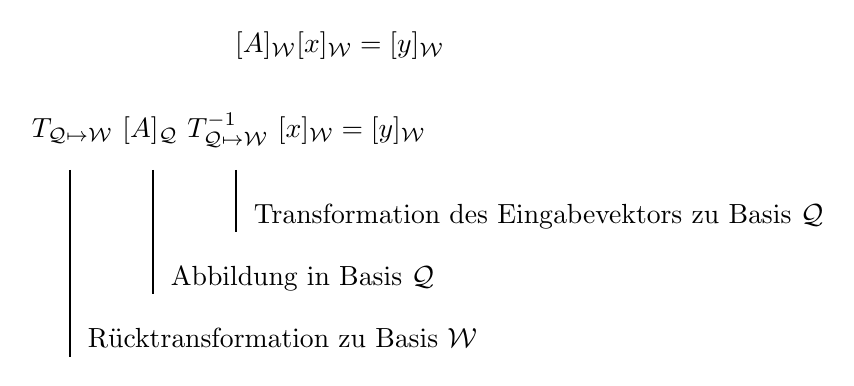
\begin{tikzpicture}[x=0.75pt,y=0.75pt,yscale=-1,xscale=1]
        %uncomment if require: \path (0,300); %set diagram left start at 0, and has height of 300
        %Straight Lines [id:da8191435773510127] 
        \draw    (370,100) -- (370,130) ;
        %Straight Lines [id:da8490818469111169] 
        \draw    (330,100) -- (330,160) ;
        %Straight Lines [id:da9710596741479948] 
        \draw    (290,100) -- (290,190) ;

        % Text Node
        \draw (368,32) node [anchor=north west][inner sep=0.75pt]   [align=left] {\( [A]_\mathcal{W} [x]_\mathcal{W} = [y]_\mathcal{W} \)};
        % Text Node
        \draw (270,71) node [anchor=north west][inner sep=0.75pt]   [align=left] {\( T_{\mathcal{Q} \mapsto \mathcal{W}} \ [A]_\mathcal{Q} \ T_{\mathcal{Q} \mapsto \mathcal{W}}^{-1} \ [x]_\mathcal{W} = [y]_\mathcal{W} \)};
        % Text Node
        \draw (377,115) node [anchor=north west][inner sep=0.75pt]   [align=left] {Transformation des Eingabevektors zu Basis \( \mathcal{Q} \)};
        % Text Node
        \draw (337,145) node [anchor=north west][inner sep=0.75pt]   [align=left] {Abbildung in Basis \( \mathcal{Q} \)};
        % Text Node
        \draw (297,175) node [anchor=north west][inner sep=0.75pt]   [align=left] {Rücktransformation zu Basis \( \mathcal{W} \)};
    \end{tikzpicture}
\end{figure}

\subsubsection*{Beispiel}

Eine Basis sei gegeben mit \( \mathcal{B} = \left\{ \begin{bmatrix} 1 \\ 2 \end{bmatrix}_\mathcal{S}, \begin{bmatrix} 0 \\ 1 \end{bmatrix}_\mathcal{S} \right\} \). Transformiere die Matrix \( [A]_\mathcal{S} = \begin{pmatrix} 3 & 1 \\ 0 & 2 \end{pmatrix} \) aus der Standardbasis \( \mathcal{S} \) in die Basis \( \mathcal{B} \).

\vspace{1\baselineskip}

Wir benutzten hier die oben eingeführte Transformationsmatrix in diesem Fall bekommen wir

\begin{equation*}
    \begin{aligned}
        [A]_\mathcal{B} &= T_{\mathcal{S} \mapsto \mathcal{B}} \ [A]_\mathcal{S} \ T_{\mathcal{S} \mapsto \mathcal{B}}^{-1} \\[1em]
        &= \begin{pmatrix} 1 & 0 \\ -2 & 1 \end{pmatrix} \begin{pmatrix} 3 & 1 \\ 0 & 2 \end{pmatrix} \begin{pmatrix} 1 & 0 \\ 2 & 1 \end{pmatrix} = \begin{pmatrix} 1 & 0 \\ -2 & 1 \end{pmatrix} \begin{pmatrix} 5 & 1 \\ 4 & 2 \end{pmatrix} = \begin{pmatrix} 5 & 1 \\ -6 & 0 \end{pmatrix}
    \end{aligned}
\end{equation*}

\subsection{Diagonalisieren}

Wir wissen nun wie wir von einer Basis zur anderen wechseln können, indem wir Vektoren und Matrizen transformieren. Da lineare Abbildungen durch Matrizen beschrieben werden können, sind wir auch in der Lage lineare Abbildungen von einer Basis in die andere zu transformieren. Für solche Abbildungen ist es vorteilhaft, wenn die dazugehörige Abbildungsmatrix diagonal ist. Denn Diagonalmatrizen sind leicht invertierbar und Matrixmultiplikation ist bedeutend unkomplizierter. Beim sogenannten Diagonalisieren wollen wir einen Basiswechsel durchführen, sodass eine gewünschte Matrix in der neuen Basis diagonal ist. Konkreter wollen wir für eine quadratische Matrix \( A \in \mathbb{C}^{n \times n} \) eine Matrix \( T \in \mathbb{C}^{n \times n} \) finden, sodass

\begin{equation*}
    T^{-1} A \ T = D = \text{diag}(d_1, d_2, \dots, d_n),
\end{equation*}

wobei \( D \) die Matrix in der neuen Basis ist. Um die Diagonalisierung durchzuführen, müssen wir demnach die Basis finden in der \( A \) diagonal ist. Dafür nehmen wir nochmals einen Schritt zurück und überlegen uns was der Effekt von diagonalen Matrizen und deren assoziierter Abbildung im zweidimensionalen Raum ist. Im folgenden Beispiel betrachten wie eine Diagonalmatrix verschiedene Vektoren im Raum abbildet.

\newpage

\begin{figure}[h]
    \centering
    \tikzset{every picture/.style={line width=0.75pt}} %set default line width to 0.75pt        

    \begin{tikzpicture}[x=0.75pt,y=0.75pt,yscale=-1,xscale=1]
        %uncomment if require: \path (0,300); %set diagram left start at 0, and has height of 300

        %Straight Lines [id:da09322443868180241] 
        \draw [color={rgb, 255:red, 0; green, 0; blue, 0 }  ,draw opacity=1 ]   (180,180) -- (180,73) ;
        \draw [shift={(180,70)}, rotate = 90] [fill={rgb, 255:red, 0; green, 0; blue, 0 }  ,fill opacity=1 ][line width=0.08]  [draw opacity=0] (5.36,-2.57) -- (0,0) -- (5.36,2.57) -- (3.56,0) -- cycle    ;
        %Straight Lines [id:da7661269003315404] 
        \draw [color={rgb, 255:red, 0; green, 0; blue, 0 }  ,draw opacity=1 ]   (160,160) -- (277,160) ;
        \draw [shift={(280,160)}, rotate = 180] [fill={rgb, 255:red, 0; green, 0; blue, 0 }  ,fill opacity=1 ][line width=0.08]  [draw opacity=0] (5.36,-2.57) -- (0,0) -- (5.36,2.57) -- (3.56,0) -- cycle    ;
        %Straight Lines [id:da8304021944367197] 
        \draw [color={rgb, 255:red, 74; green, 144; blue, 226 }  ,draw opacity=1 ][line width=1.5]    (180,160) -- (216,160) ;
        \draw [shift={(220,160)}, rotate = 180] [fill={rgb, 255:red, 74; green, 144; blue, 226 }  ,fill opacity=1 ][line width=0.08]  [draw opacity=0] (6.43,-3.09) -- (0,0) -- (6.43,3.09) -- (4.27,0) -- cycle    ;
        %Straight Lines [id:da191012214368245] 
        \draw [color={rgb, 255:red, 208; green, 2; blue, 27 }  ,draw opacity=1 ][line width=1.5]    (180,160) -- (180,124) ;
        \draw [shift={(180,120)}, rotate = 90] [fill={rgb, 255:red, 208; green, 2; blue, 27 }  ,fill opacity=1 ][line width=0.08]  [draw opacity=0] (6.43,-3.09) -- (0,0) -- (6.43,3.09) -- (4.27,0) -- cycle    ;
        %Straight Lines [id:da09698667695537988] 
        \draw [color={rgb, 255:red, 126; green, 211; blue, 33 }  ,draw opacity=1 ][line width=1.5]    (180,160) -- (199.03,83.88) ;
        \draw [shift={(200,80)}, rotate = 104.04] [fill={rgb, 255:red, 126; green, 211; blue, 33 }  ,fill opacity=1 ][line width=0.08]  [draw opacity=0] (6.43,-3.09) -- (0,0) -- (6.43,3.09) -- (4.27,0) -- cycle    ;
        %Straight Lines [id:da4000741652473213] 
        \draw [color={rgb, 255:red, 0; green, 0; blue, 0 }  ,draw opacity=1 ]   (440,180) -- (440,73) ;
        \draw [shift={(440,70)}, rotate = 90] [fill={rgb, 255:red, 0; green, 0; blue, 0 }  ,fill opacity=1 ][line width=0.08]  [draw opacity=0] (5.36,-2.57) -- (0,0) -- (5.36,2.57) -- (3.56,0) -- cycle    ;
        %Straight Lines [id:da1897122839365225] 
        \draw [color={rgb, 255:red, 0; green, 0; blue, 0 }  ,draw opacity=1 ]   (420,160) -- (537,160) ;
        \draw [shift={(540,160)}, rotate = 180] [fill={rgb, 255:red, 0; green, 0; blue, 0 }  ,fill opacity=1 ][line width=0.08]  [draw opacity=0] (5.36,-2.57) -- (0,0) -- (5.36,2.57) -- (3.56,0) -- cycle    ;
        %Straight Lines [id:da5005263479036821] 
        \draw [color={rgb, 255:red, 74; green, 144; blue, 226 }  ,draw opacity=1 ][line width=1.5]    (440,160) -- (516,160) ;
        \draw [shift={(520,160)}, rotate = 180] [fill={rgb, 255:red, 74; green, 144; blue, 226 }  ,fill opacity=1 ][line width=0.08]  [draw opacity=0] (6.43,-3.09) -- (0,0) -- (6.43,3.09) -- (4.27,0) -- cycle    ;
        %Straight Lines [id:da006942301425049924] 
        \draw [color={rgb, 255:red, 208; green, 2; blue, 27 }  ,draw opacity=1 ][line width=1.5]    (440,160) -- (440,144) ;
        \draw [shift={(440,140)}, rotate = 90] [fill={rgb, 255:red, 208; green, 2; blue, 27 }  ,fill opacity=1 ][line width=0.08]  [draw opacity=0] (6.43,-3.09) -- (0,0) -- (6.43,3.09) -- (4.27,0) -- cycle    ;
        %Straight Lines [id:da5276888984657642] 
        \draw [color={rgb, 255:red, 126; green, 211; blue, 33 }  ,draw opacity=1 ][line width=1.5]    (440,160) -- (477.17,122.83) ;
        \draw [shift={(480,120)}, rotate = 135] [fill={rgb, 255:red, 126; green, 211; blue, 33 }  ,fill opacity=1 ][line width=0.08]  [draw opacity=0] (6.43,-3.09) -- (0,0) -- (6.43,3.09) -- (4.27,0) -- cycle    ;
        %Straight Lines [id:da5424500359174866] 
        \draw [color={rgb, 255:red, 0; green, 0; blue, 0 }  ,draw opacity=1 ]   (320,120) -- (387,120) ;
        \draw [shift={(390,120)}, rotate = 180] [fill={rgb, 255:red, 0; green, 0; blue, 0 }  ,fill opacity=1 ][line width=0.08]  [draw opacity=0] (5.36,-2.57) -- (0,0) -- (5.36,2.57) -- (3.56,0) -- cycle    ;

        % Text Node
        \draw (305,65) node [anchor=north west][inner sep=0.75pt]   [align=left] {\( A = \begin{pmatrix} 2 & 0 \\ 0 & 0.5 \end{pmatrix} \)};
    \end{tikzpicture}
\end{figure}

\begin{equation*}
    \begin{pmatrix} 2 & 0 \\ 0 & \frac{1}{2} \end{pmatrix} \begin{bmatrix} 1 \\ 0 \end{bmatrix} = \begin{bmatrix} 2 \\ 0 \end{bmatrix}, \quad \begin{pmatrix} 2 & 0 \\ 0 & \frac{1}{2} \end{pmatrix} \begin{bmatrix} 0 \\ 1 \end{bmatrix} = \begin{bmatrix} 0 \\ \frac{1}{2} \end{bmatrix}
\end{equation*}

\vspace{0.25\baselineskip}

Wir erkennen, dass die Basisvektoren (hier die Standardbasis in Blau und Rot) nur skaliert werden, aber nicht Ihre Richtung ändern. Das ist genau wie bei Eigenvektoren. In anderen Worten sind bei Diagonalmatrizen die Eigenvektoren auch die Basisvektoren. Indem wir also die Eigenvektoren der ursprünglichen Matrix als neue Basisvektoren wählen, garantieren wir, dass die Matrix in der neuen Basis diagonal ist. Weiterhin sehen wir, dass die Diagonaleinträge der Matrix genau die Faktoren sind mit denen die Basisvektoren skaliert werden. D.h.\ die Diagonaleinträge der diagonalisierten Matrix sind auch die Eigenwerte der ursprünglichen Matrix.

\vspace{1\baselineskip}

Sei zum Beispiel eine Matrix A in der Standardbasis \( \mathcal{S} \) gegeben durch \( A = \begin{pmatrix} 2 & -1 \\ 0 & 1 \end{pmatrix} \). Weiter seinen die Eigenwerte und Eigenvektoren von \( A \) gegeben durch

\begin{equation*}
    \lambda_1 = 2, \quad v_1 = \begin{bmatrix} 1 \\ 0 \end{bmatrix}, \quad \lambda_2 = 1, \quad v_2 = \begin{bmatrix} 1 \\ 1 \end{bmatrix}.
\end{equation*}

Um \( A \) zu diagonalisieren suchen wir eine Basis \( \mathcal{B} \), in der die Basisvektoren durch die Eigenvektoren \( v_1, v_2 \) gegeben sind. Anschliessend benötigen wir nur noch eine Transformationsmatrix, um in die entsprechende Basis zu wechseln. Mit den gegebenen Eigenvektoren können wir bereits die Übergangsmatrix \( T_{\mathcal{B} \mapsto \mathcal{S} } \) bestimmen, indem wir die Eigenvektoren als Spalten nehmen:

\begin{equation*}
    T_{\mathcal{B} \mapsto \mathcal{S} } = \begin{pmatrix} 1 & 1 \\ 0 & 1 \end{pmatrix}.
\end{equation*}

Die diagonalisierte Matrix \( D \) ist dann gegeben durch

\begin{equation*}
    D = T_{\mathcal{B} \mapsto \mathcal{S} }^{-1} \ A \ T_{\mathcal{B} \mapsto \mathcal{S} } = \begin{pmatrix} 2 & 0 \\ 0 & 1 \end{pmatrix}.
\end{equation*}

Die Eigenwerte der Matrix \( A \) sind nun auch die Diagonaleinträge der Matrix \( D \). Gleichermassen gilt auch 

\begin{equation*}
    A = T_{\mathcal{B} \mapsto \mathcal{S} } \ D \ T_{\mathcal{B} \mapsto \mathcal{S} }^{-1}.
\end{equation*}

Zusammengefasst können wir dies in einem ``Kochrezept'' aufschreiben.

\begin{tcolorbox}[colback=gray!30, colframe=gray!80, title=Diagonalisieren]
    Um eine Matrix \( A \in \mathbb{C}^{n \times n} \) zu diagonalisieren (\( D = T^{-1}AT \)), gehe wie folgt vor:
    \begin{enumerate}
        \item Bestimme die Eigenwerte \( \lambda_i \) und Eigenvektoren \( v_i \) von \( A \).
        \item Die Matrix \( D = \text{diag}(\lambda_1, \dots , \lambda_n) \) ist die diagonalisierte Matrix.
        \item Setze die Eigenvektoren als Spalten in die Matrix \( T \) ein (\textbf{Gleiche Reihenfolge wie bei \( \mathbf{D} \)!}).
        \item Bestimme \( T^{-1} \). Falls Eigenvektoren orthonormal sind, gilt: \( T^{-1} = T^\top \).
    \end{enumerate}
\end{tcolorbox}

\subsection{Diagonalisierbarkeit}

Nicht alle Matrizen sind Diagonalisierbar. Um zu prüfen, ob eine Matrix diagonalisierbar ist, können wir bestimmte Kriterien überprüfen. Erinnern wir uns nochmals wie die Diagonalisierung aussieht mathematisch aussieht,

\begin{equation*}
    D = T^{-1} A T.
\end{equation*}

Ein Kriterium ist damit gegeben, dass die Transformationsmatrix \( T \) regulär (invertierbar) sein muss. Ein Weg die Invertierbarkeit einer Matrix zu prüfen ist die lineare Abhängigkeit der Spalten/ Zeilen zu betrachten. Nur wenn alle Spalten linear unabhängig sind, ist die Matrix auch invertierbar. In diesem Fall sind die Spalten der Matrix \( T \) auch die Eigenvektoren von \( A \). Das bedeutet, dass wir prüfen müssen, ob die Eigenvektoren von \( A \) linear unabhängig sind. Dieses Kriterium können wir leicht umschreiben denn, wenn alle Eigenvektoren linear unabhängig sind dann bilden sie auch eine Basis. Wenn das der Fall ist, dann sagen wir das die Matrix halbeinfach ist. 

\begin{tcolorbox}[colback=gray!30, colframe=gray!80, title=Halbeinfache Matrizen]
    Eine Matrix \( A \in \mathbb{C}^{n \times n} \) ist halbeinfach, wenn Ihre Eigenvektoren eine Basis für \( \mathbb{C}^n \) bilden. 
\end{tcolorbox}

Weiterhin können wir prüfen, ob eine Matrix halbeinfach ist, indem wir uns die Vielfachheiten der Eigenwerte und Eigenvektoren anschauen. Nur wenn die algebraische Vielfachheit jedes Eigenwertes gleich der geometrischen Vielfachheit ist, ist die Matrix halbeinfach. D.h. für jeden Eigenwert \( \lambda \) muss gelten:

\begin{equation*}
    \text{alg. Vfh. } \lambda = \text{geom. Vfh. } \lambda.
\end{equation*}

Somit können wir das Kriterium für die Diagonalisierbarkeit einer Matrix zusammenfassen.

\begin{tcolorbox}[colback=gray!30, colframe=gray!80, title=Halbeinfache Matrizen]
    Eine quadratische Matrix \( A \in \mathbb{C}^{n \times n} \) ist diagonalisierbar, falls eine reguläre Matrix \( T \) existiert, sodass \( D = T^{-1} A T \) eine Diagonalmatrix ist. 

    \begin{equation*}
        A \ \text{halbeinfach} \Leftrightarrow A \ \text{diagonalisierbar}
    \end{equation*}
\end{tcolorbox}

\subsubsection*{Beispiel} \( \ \)

Halbeinfache Martix: \( A = \begin{pmatrix} 2 & -1 \\ 0 & 1 \end{pmatrix} \). Mit den Eigenwerten und Eigenvektoren

\vspace{1\baselineskip}

\begin{equation*}
    \lambda_1 = 2, \ \lambda_2 = 1, \quad v_1 = \begin{bmatrix} 1 \\ 0 \end{bmatrix}, \ v_2 = \begin{bmatrix} 1 \\ 1 \end{bmatrix}.
\end{equation*}

In diesem Fall sind alle geometrischen und algebraischen Vielfachheiten gleich 1 damit bilden die Eigenvektoren eine Basis. Die Matrix ist also halbeinfach und damit auch diagonalisierbar.

\vspace{1\baselineskip}

Nicht halbeinfache Martix: \( A = \begin{pmatrix} 1 & 1 \\ -1 & 3 \end{pmatrix} \). Mit den Eigenwerten und Eigenvektoren

\vspace{1\baselineskip}

\begin{equation*}
    \lambda_{1,2} = 2, \quad v_1 = \begin{bmatrix} 1 \\ 1 \end{bmatrix}.
\end{equation*}

Hier ist die algebraische Vielfachheit des Eigenwertes 2 gleich 2, aber die geometrische Vielfachheit nur gliech 1 damit bilden die Eigenvektoren keine Basis. Dmenach ist die Matrix nicht halbeinfach und damit auch nicht diagonalisierbar.

\subsubsection{Spezialfall: Symmetrische Matrizen} \( \ \)

\vspace{0.5\baselineskip}

Wenn \( A \in \mathbb{R}^{n \times n} \)  symmetrisch ist das gilt:

\begin{itemize}
    \item A ist halbeinfach, also auch diagonalisierbar.
    \item A besitzt eine orthnormale Eigenbasis.
    \item Es exsistiert eine orthogonale Matrix \( T \), sodass \( T^{-1} A T = T^\top A T \) diagonal ist.
\end{itemize}

\subsubsection{Anwendung: Potenzen von Matrizen} \( \ \)

\vspace{0.5\baselineskip}

Sei \( A \in \mathbb{C}^{n \times n} \) diagonalisierbar. Berechne \( A^3 \). 

\vspace{1\baselineskip}

Da \( A \) diagonalisierbar ist gilt \( A = T D T^{-1} \). Damit gilt für \( A^3 \):

\begin{equation*}
    \begin{aligned}
        A^3 &= (T D T^{-1})^3 = T D \underbrace{T^{-1} T}_{I} D \underbrace{T^{-1} T}_{I} D T^{-1} = T D^3 \ T^{-1}.
    \end{aligned}
\end{equation*} 

und weil \( D \) eine Diagonalmatrix ist, gilt

\begin{equation*}
    D^3 = T \ \text{diag}(\lambda_1^3, \lambda_2^3, \dots, \lambda_n^3) \ T^{-1}.
\end{equation*}

Allgemein gilt für jede diagonalisierbare Matrix \( A \)

\begin{equation*}
    A^k = T \ \text{diag}(\lambda_1^k, \lambda_2^k, \dots, \lambda_n^k) \ T^{-1}.
\end{equation*}

Insbesondre vereinfacht sich dadurch auch das Matrixpotential

\begin{equation*}
    e^{At} \underset{\substack{\color{black}\uparrow \\
                       \mathclap{e^A = \sum_{m=0}^{\infty} \frac{A^m}{m!}}}}{=}T \ \text{diag}(e^{\lambda_1 t}, e^{\lambda_2 t}, \dots, e^{\lambda_n t}) \ T^{-1}
\end{equation*}